\documentclass[10pt, aspectratio=169, handout]{beamer}
\usefonttheme{professionalfonts}
%\usetheme{CambridgeUS}
%
% Choose how your presentation looks.
%
% For more themes, color themes and font themes, see:
% http://deic.uab.es/~iblanes/beamer_gallery/index_by_theme.html
%
\mode<presentation>
{
  \usetheme{Berkeley}      % or try Darmstadt, Madrid, Warsaw, ...
  \usecolortheme{beaver} % or try albatross, beaver, crane, ...
  \usefonttheme{default}  % or try serif, structurebold, ...
  \setbeamertemplate{navigation symbols}{}
  \setbeamertemplate{caption}[numbered]
} 

\setbeamertemplate{footline}{%
  \leavevmode%
  \hbox{%
    \begin{beamercolorbox}[wd=.85\paperwidth,ht=2.5ex,dp=1ex,left]{author in head/foot}%
      \usebeamerfont{author in head/foot}Digital Signal Processing, Fall 2025%
    \end{beamercolorbox}%
    \begin{beamercolorbox}[wd=.15\paperwidth,ht=2.5ex,dp=1ex,right]{date in head/foot}%
      \hspace*{0.5em}\insertframenumber{} / \inserttotalframenumber\hspace*{0.5em}%
    \end{beamercolorbox}%
  }%
  \vskip0pt%
}

\usepackage[english]{babel}
\usepackage[utf8x]{inputenc}
\usepackage{tikz}
\usepackage{pgfplots}
\usepackage{array}  % for table column M
\usepackage{makecell} % to break line within a cell
\usepackage{verbatim}
\usepackage{graphicx}
\usepackage{subcaption}
\usepackage{amsfonts}
\usepackage{amsmath}
\usepackage{bm}
\usepackage{epstopdf}
\usepackage{ifthen}
\captionsetup{compatibility=false}
%\usepackage{dsfont}
\usepackage[absolute,overlay]{textpos}
\usepackage{ifthen}

\usetikzlibrary{calc}
\usetikzlibrary{pgfplots.fillbetween, backgrounds}
\usetikzlibrary{positioning}

\newboolean{showresults}
\setboolean{showresults}{true}

\usetikzlibrary{pgfplots.groupplots}
\usetikzlibrary{plotmarks}
\usetikzlibrary{calc}

\usepgfplotslibrary{groupplots}
\pgfplotsset{compat=newest} 
%\pgfplotsset{plot coordinates/math parser=false}

\usepackage{hyperref}
\hypersetup{
    colorlinks=true,
    linkcolor=blue,
    filecolor=magenta,      
    urlcolor=cyan,
}


% %% 
% \input{header.tex}

% %%
\title[ECEN 463/863]{Discrete Time Systems and Properties}
\author{Maxx Seminario}
\institute{University of Nebraska-Lincoln}
\date{September 1, 2025}

\begin{document}
\begin{frame}
  \titlepage
\end{frame}

\section{Introduction}

\begin{frame}{What is a Discrete-Time System?}
\begin{itemize}
    \item A \textbf{discrete-time system} is mathematically defined as a transformation or operator that maps an input sequence $x[n]$ into an output sequence $y[n]$.
    \item This can be denoted as:
    \[
        y[n] = T\{x[n]\}
    \]
    \item $T\{\cdot\}$ represents a rule or formula for computing output values from input values.
    \item The output $y[n]$ at each index $n$ may depend on all or part of the entire input sequence $x[n]$.
\end{itemize}
\end{frame}

\begin{frame}{Pictorial Representation}
\begin{center}
    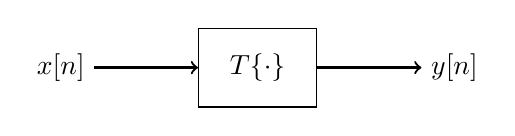
\begin{tikzpicture}[node distance=2.5cm]
        \node (x) {$x[n]$};
        \node [draw, rectangle, right of=x, minimum width=1.5cm, minimum height=1cm] (T) {$T\{\cdot\}$};
        \node [right of=T] (y) {$y[n]$};
        \draw[->, thick] (x) -- (T);
        \draw[->, thick] (T) -- (y);
    \end{tikzpicture}
\end{center}
\begin{itemize}
    \item The system transforms the input sequence $x[n]$ into a unique output sequence $y[n]$.
\end{itemize}
\end{frame}

\begin{frame}{Example 1: The Ideal Delay System}
\begin{itemize}
    \item The \textbf{ideal delay system} is defined by:
    \[
        y[n] = x[n-n_d], \quad -\infty < n < \infty
    \]
    \item $n_d$ is a fixed positive integer representing the delay.
    \item The system shifts the input sequence to the right by $n_d$ samples.
    \item If $n_d$ is negative, the system shifts the input to the left by $|n_d|$ samples (time advance).
\end{itemize}
\end{frame}

\begin{frame}{Example 2: Moving Average System}
\begin{itemize}
    \item The \textbf{moving-average system} is defined by:
    \[
        y[n] = \frac{1}{M_1 + M_2 + 1} \sum_{k=-M_1}^{M_2} x[n-k]
    \]
    \item $M_1$ and $M_2$ are non-negative integers.
    \item This system computes $y[n]$ as the average of $(M_1 + M_2 + 1)$ samples of $x[n]$ around index $n$.
\end{itemize}
\end{frame}

\begin{frame}{Moving Average: Visualization}
\begin{center}
    \begin{tikzpicture}[scale=1]
        % Dotted region for involved samples
        \draw[dotted, thick] (1,0) -- (1,2.2);
        \draw[dotted, thick] (6,0) -- (6,2.2);
        % Axis
        \draw[->] (0,0) -- (7.5,0) node[right] {$k$};
        \draw[->] (0,0) -- (0,2.5) node[above] {$x[k]$};
        % Stem plot
        \foreach \k/\x in {1/1.3, 2/2.1, 3/1.8, 4/1.0, 5/1.5, 6/2.0, 7/0.9} {
            \ifnum\k>0
                \draw[thick] (\k,0) -- (\k,\x);
                \filldraw[blue] (\k,\x) circle (2pt);
            \fi
        }
        % Mark n
        \draw[thick, red] (6,-0.15) -- (6,0.15);
        \node[below, red] at (6,-0.15) {$n$};
        % Mark n-5 for M2=5, M1=0
        \draw[thick, red] (1,-0.15) -- (1,0.15);
        \node[below, red] at (1,-0.15) {$n-5$};
    \end{tikzpicture}
\end{center}
\begin{itemize}
    \item For $n=7$, $M_1=0$, $M_2=5$: $y[7]$ is the average of the six samples from $n-5$ to $n$.
    \item To compute $y[8]$, the region shifts right by one sample.
\end{itemize}
\end{frame}


\begin{frame}{Example 3: Accumulator System}
\begin{itemize}
    \item \textbf{Accumulator system:}
    \[
        y[n] = \sum_{k=-\infty}^{n} x[k]
    \]
    \item \textbf{Analog Circuit Equivalent:}
    \begin{itemize}
        \item The voltage across a capacitor is proportional to the total charge stored:
        \[
            v_C(t) = \frac{1}{C} q(t)
        \]

        \[
            q(t) = \int_{-\infty}^t i(\tau) \, d\tau
        \]

        \[
            v_C(t) = \frac{1}{C} \int_{-\infty}^t i(\tau) \, d\tau
        \]
    \end{itemize}
    \item The accumulator sums, just as a capacitor integrates current to produce voltage.
\end{itemize}
\end{frame}


\begin{frame}{Classes of Discrete-Time Systems}
\begin{itemize}
    \item Different classes of systems are defined by placing constraints on the properties of the transformation $T\{\cdot\}$.
    \item These constraints often lead to general mathematical representations.
    \item Of particular importance are system properties such as linearity, time-invariance, causality, stability, and memory.
\end{itemize}
\end{frame}

\section{Memory}

\begin{frame}{Memoryless Systems}
\begin{itemize}
    \item A system is \textbf{memoryless} if the output $y[n]$ at each $n$ depends only on the input $x[n]$ at the same $n$.
    \item $y[n] = (x[n])^2$ is memoryless.
 \item The ideal delay system and the moving average system are \textbf{not} memoryless unless $n_d=0$ or $M_1=M_2=0$, respectively.
    \[
        \text{Ideal delay:} \quad y[n] = x[n-n_d]
    \]
    \[
        \text{Moving average:} \quad y[n] = \frac{1}{M_1+M_2+1} \sum_{k=-M_1}^{M_2} x[n-k]
    \]
\end{itemize}
\end{frame}

\section{Linearity}

\begin{frame}{Linear Systems}
\begin{itemize}
    \item A system is \textbf{linear} if it satisfies the \emph{principle of superposition}:
    \begin{align*}
        &T\{x_1[n] + x_2[n]\} = T\{x_1[n]\} + T\{x_2[n]\} \\
        &T\{a x[n]\} = a T\{x[n]\}
    \end{align*}
    \item In general, for any sequences $x_k[n]$ and scalars $a_k$:
    \[
        T\left\{\sum_k a_k x_k[n]\right\} = \sum_k a_k T\{x_k[n]\}
    \]
\end{itemize}
\end{frame}

\begin{frame}{Is the Ideal Delay System Linear?}
\begin{itemize}
    \item Consider the system $y[n] = x[n - n_d]$.
    \item Question: Is this system linear?
    \item What happens if we input a linear combination $a x_1[n] + b x_2[n]$?
    \item Does the output satisfy $T\{a x_1[n] + b x_2[n]\} = a T\{x_1[n]\} + b T\{x_2[n]\}$?
\end{itemize}
\end{frame}

\ifthenelse{\boolean{showresults}}{
\begin{frame}{Linearity: Ideal Delay System}
\begin{itemize}
    \item \textbf{Definition:} $y[n] = x[n - n_d]$
    \item \textbf{Test for Linearity:}
    \begin{itemize}
        \item For inputs $x_1[n]$ and $x_2[n]$, and scalars $a, b$:
        \[
            T\{a x_1[n] + b x_2[n]\} = a T\{x_1[n]\} + b T\{x_2[n]\}
        \]
        \item Compute:
        \[
            T\{a x_1[n] + b x_2[n]\} = a x_1[n - n_d] + b x_2[n - n_d] = a T\{x_1[n]\} + b T\{x_2[n]\}
        \]
    \end{itemize}
    \item \textbf{Conclusion:} The ideal delay system is linear.
\end{itemize}
\end{frame}
}{}

\begin{frame}{Is the Moving Average System Linear?}
\begin{itemize}
    \item Consider the system:
    \[
        y[n] = \frac{1}{M_1 + M_2 + 1} \sum_{k=-M_1}^{M_2} x[n - k]
    \]
    \item Question: Is this system linear?
    \item What happens for the input $a x_1[n] + b x_2[n]$?
    \item Does the system satisfy the superposition property?
\end{itemize}
\end{frame}

\ifthenelse{\boolean{showresults}}{
\begin{frame}{Linearity: Moving Average System}
\begin{itemize}
    \item \textbf{Definition:}
    \[
        y[n] = \frac{1}{M_1 + M_2 + 1} \sum_{k=-M_1}^{M_2} x[n - k]
    \]
    \item \textbf{Test for Linearity:}
    \begin{itemize}
        \item For $x_1[n]$, $x_2[n]$, $a$, $b$:
        \[
            T\{a x_1[n] + b x_2[n]\} = \frac{1}{M_1 + M_2 + 1} \sum_{k=-M_1}^{M_2} \left[ a x_1[n - k] + b x_2[n - k] \right]
        \]
        \item This expands to:
        \[
            a T\{x_1[n]\} + b T\{x_2[n]\}
        \]
    \end{itemize}
    \item \textbf{Conclusion:} The moving average system is linear.
\end{itemize}
\end{frame}
}{}


\begin{frame}{Is $y[n] = (x[n])^2$ Linear?}
\begin{itemize}
    \item Consider the system $y[n] = (x[n])^2$.
    \item Question: Is this system linear?
    \item What happens if we input $x_1[n] + x_2[n]$?
    \item Does the output satisfy the superposition property?
\end{itemize}
\end{frame}

\ifthenelse{\boolean{showresults}}{
\begin{frame}{Why is $y[n] = (x[n])^2$ Not Linear?}
\begin{itemize}
    \item \textbf{Definition:} $y[n] = (x[n])^2$
    \item \textbf{Test for Linearity:}
    \begin{itemize}
        \item For $x_1[n]$ and $x_2[n]$:
        \[
            T\{x_1[n] + x_2[n]\} = (x_1[n] + x_2[n])^2 = (x_1[n])^2 + 2x_1[n]x_2[n] + (x_2[n])^2
        \]
        \item $T\{x_1[n]\} + T\{x_2[n]\} = (x_1[n])^2 + (x_2[n])^2$
    \end{itemize}
    \item \textbf{Conclusion:} Extra cross-term $2x_1[n]x_2[n]$ means the system is \textbf{not} linear.
    \item In other words, this cross-term is a second-order nonlinearity, where the two inputs, $x_1[n]$ and $x_2[n]$, mix to produce an output component that depends on both signals simultaneously.
\end{itemize}
\end{frame}
}{}


\begin{frame}{Is the Accumulator System Linear?}
\begin{itemize}
    \item Consider the accumulator system:
    \[
        y[n] = \sum_{k=-\infty}^{n} x[k]
    \]
    \item Question: Is this system linear?
    \item If we input a linear combination, does the output satisfy the superposition property?
\end{itemize}
\end{frame}

\ifthenelse{\boolean{showresults}}{
\begin{frame}{Linearity: The Accumulator System}
    \[
    y[n] = \sum_{k=-\infty}^{n} x[k]
    \]
\begin{itemize}
    \item The output at time $n$ is the sum of all present and past input samples.
    \item This system is linear:
    \begin{align*}
        y_1[n] &= \sum_{k=-\infty}^{n} x_1[k] \\
        y_2[n] &= \sum_{k=-\infty}^{n} x_2[k] \\
        y_3[n] &= \sum_{k=-\infty}^{n} (a x_1[k] + b x_2[k]) = a y_1[n] + b y_2[n]
    \end{align*}
\end{itemize}
\end{frame}
}{}

\begin{frame}{Example: A Nonlinear System}
\begin{itemize}
    \item Consider $w[n] = \log_{10}(|x[n]|)$.
    \item This system is \textbf{not} linear.
    \item Counterexample: $x_1[n]=1$, $x_2[n]=10$.
    \begin{itemize}
        \item $w_1[n] = 0$, $w_2[n] = 1$
        \item $w[n]$ for $x_1[n]+x_2[n]=11$: $\log_{10}(11) \neq \log_{10}(1) + \log_{10}(10)$
        \item Scaling property also fails: $w_2[n] \neq 10 w_1[n]$
    \end{itemize}
\end{itemize}
\end{frame}

\section{Time-Invariance}

\begin{frame}{Time-Invariant Systems}
\begin{itemize}
    \item A system is \textbf{time-invariant} if a shift in the input causes an identical shift in the output.
    \item If $x_1[n] = x[n-n_0]$, then $y_1[n] = y[n-n_0]$ for all $n_0$.
    \item All previously studied systems are time invariant.
\end{itemize}
\end{frame}

\begin{frame}{Time-Invariance: The Accumulator}
\begin{itemize}
    \item For accumulator: $y[n] = \sum_{k=-\infty}^{n} x[k]$
    \item For shifted input $x_1[n] = x[n-n_0]$:
    \[
        y_1[n] = \sum_{k=-\infty}^n x[k-n_0]
    \]
    \item Change variable $k_1 = k - n_0$:
    \[
        y_1[n] = \sum_{k_1=-\infty}^{n-n_0} x[k_1] = y[n-n_0]
    \]
    \item Thus, the accumulator is time-invariant.
\end{itemize}
\end{frame}

\begin{frame}{Time-Invariance: The Compressor}
    \[
        y[n] = x[Mn], \quad M > 0
    \]
\begin{itemize}
    \item $M$ compresses the input by keeping every $M$th sample and discarding the rest
    \item Shift input: $x_1[n] = x[n-n_0]$
    \[
        y_1[n] = x_1[Mn] = x[Mn - n_0]
    \]
    \item Delay output: 
    \[
        y[n-n_0] = x[M(n-n_0)]
    \]
    \item $x[Mn - n_0] \neq x[M(n-n_0)]$ in general
    \item Not time-invariant
\end{itemize}
\end{frame}

\section{Causality}
% --- Causality Slides ---

\begin{frame}{Causality Definition}
\begin{itemize}
    \item A system is \textbf{causal} if the output at time $n_0$ depends only on input values for $n \leq n_0$.
    \item If $x_1[n] = x_2[n]$ for $n \leq n_0$, then $y_1[n] = y_2[n]$ for $n \leq n_0$.
    \item Causal systems are non-anticipative.
\end{itemize}
\end{frame}

\begin{frame}{Causality of Previously Studied Systems}
\begin{itemize}
    \item \textbf{Ideal delay:} \quad $y[n] = x[n - n_d]$ \\
    % Causal if $n_d \geq 0$, noncausal if $n_d < 0$.
    
    \item \textbf{Moving average:} \quad $y[n] = \frac{1}{M_1 + M_2 + 1} \sum_{k=-M_1}^{M_2} x[n-k]$ \\
    % Causal if $-M_1 \geq 0$ and $M_2 \geq 0$.
    
    \item \textbf{Squaring system:} \quad $y[n] = (x[n])^2$ \\
    % Always causal.
    
    \item \textbf{Accumulator:} \quad $y[n] = \sum_{k=-\infty}^{n} x[k]$ \\
    % Always causal.
    
    \item \textbf{Compressor:} \quad $y[n] = x[Mn]$ \\
    % Noncausal if $M > 1$.
\end{itemize}
\end{frame}

\ifthenelse{\boolean{showresults}}{
\begin{frame}{Causality of Previously Studied Systems}
\begin{itemize}
    \item \textbf{Ideal delay:} \quad $y[n] = x[n - n_d]$ \\
    Causal if $n_d \geq 0$, noncausal if $n_d < 0$.
    
    \item \textbf{Moving average:} \quad $y[n] = \frac{1}{M_1 + M_2 + 1} \sum_{k=-M_1}^{M_2} x[n-k]$ \\
    Causal if $-M_1 \geq 0$ and $M_2 \geq 0$.
    
    \item \textbf{Squaring system:} \quad $y[n] = (x[n])^2$ \\
    Always causal.
    
    \item \textbf{Accumulator:} \quad $y[n] = \sum_{k=-\infty}^{n} x[k]$ \\
    Always causal.
    
    \item \textbf{Compressor:} \quad $y[n] = x[Mn]$ \\
    Noncausal if $M > 1$.
\end{itemize}
\end{frame}
}{}

\begin{frame}{Causality: Forward and Backward Difference}
\begin{itemize}
    \item Forward difference: $y[n] = x[n+1] - x[n]$ \\
     Not causal, depends on future input.
    \item Backward difference: $y[n] = x[n] - x[n-1]$ \\
     Causal, depends only on present and past input.
\end{itemize}
\end{frame}

\begin{frame}{Causality: Forward Difference Counterexample}
\begin{itemize}
    \item Inputs: $x_1[n] = \delta[n-1]$, $x_2[n]=0$
    \item Outputs: $y_1[n] = \delta[n] - \delta[n-1]$, $y_2[n] = 0$
    \item $x_1[n]=x_2[n]$ for $n \leq 0$, but $y_1[0] \neq y_2[0]$
    \item Thus, forward difference is not causal.
\end{itemize}
\end{frame}

% --- Stability Slides ---
\section{Stability}

\begin{frame}{Stability: Definition (BIBO)}
\begin{itemize}
    \item A system is \textbf{bounded-input bounded-output (BIBO) stable} if every bounded input produces a bounded output.
    \item If $|x[n]| \leq B_x < \infty$ for all $n$, \\
    then $|y[n]| \leq B_y < \infty$ for all $n$.
    \item If any bounded input leads to unbounded output, the system is not stable.
\end{itemize}
\end{frame}

\begin{frame}{Stability: Previously Discussed Systems}
\begin{itemize}
    \item \textbf{Squaring system:} \quad $y[n] = (x[n])^2$
    \item \textbf{Logarithmic system:} \quad $y[n] = \log_{10}|x[n]|$
    \item \textbf{Accumulator:} \quad $y[n] = \sum_{k=-\infty}^n x[k]$
    \item \textbf{Moving average:} \quad $y[n] = \frac{1}{M_1 + M_2 + 1} \sum_{k=-M_1}^{M_2} x[n - k]$
    \item \textbf{Delay:} \quad $y[n] = x[n - n_d]$
    \item \textbf{Compressor:} \quad $y[n] = x[Mn]$
    \item \textbf{Forward difference:} \quad $y[n] = x[n+1] - x[n]$
    \item \textbf{Backward difference:} \quad $y[n] = x[n] - x[n-1]$
\end{itemize}
\end{frame}


\ifthenelse{\boolean{showresults}}{
\begin{frame}{Stability: Previously Discussed Systems Results}
\begin{itemize}
    \item \textbf{Squaring system:} Stable ($|y[n]| \leq B_x^2$ for bounded $x[n]$)
    \item \textbf{Logarithmic system:} Unstable ($x[n]=0$ gives $y[n] = -\infty$)
    \item \textbf{Accumulator:} Unstable (e.g., for $x[n]=u[n]$, $y[n]=n+1$ unbounded)
    \item \textbf{Moving average:} Stable (output is an average of finitely many bounded values).
    \item \textbf{Delay:} Stable (output is a shifted version of bounded input).
    \item \textbf{Compressor:} Stable (output samples are from bounded input).
    \item \textbf{Forward/Backward diff:} Stable (difference of two bounded values).
\end{itemize}
\end{frame}
}{}

\begin{frame}{Summary of System Properties}
\begin{itemize}
    \item \textbf{Memory:}
    \begin{itemize}
        \item A system is memoryless if the output $y[n]$ at each $n$ depends only on the input $x[n]$ at the same $n$.
    \end{itemize}
    \item \textbf{Linearity:}
    \begin{itemize}
        \item A system is linear if it satisfies the principle of superposition:
        \[
            T\{a_1 x_1[n] + a_2 x_2[n]\} = a_1 T\{x_1[n]\} + a_2 T\{x_2[n]\}
        \]
    \end{itemize}
    \item \textbf{Time-Invariance:}
    \begin{itemize}
        \item A system is time-invariant if a shift in the input signal causes the same shift in the output:
        \[
            x_1[n] = x[n - n_0] \implies y_1[n] = y[n - n_0]
        \]
    \end{itemize}
    \item \textbf{Causality:}
    \begin{itemize}
        \item A system is causal if the output at time $n_0$ depends only on the input values for $n \leq n_0$.
    \end{itemize}
    \item \textbf{Stability (BIBO):}
    \begin{itemize}
        \item A system is bounded-input bounded-output (BIBO) stable if every bounded input produces a bounded output:
        \[
            |x[n]| \leq B_x < \infty \implies |y[n]| \leq B_y < \infty
        \]
    \end{itemize}
\end{itemize}
\end{frame}


\end{document}
